\documentclass[10pt,twocolumn,letterpaper]{article}

\usepackage{cvpr}
\usepackage{times}
\usepackage{epsfig}
\usepackage{graphicx}
\usepackage{amsmath}
\usepackage{amssymb}

% Include other packages here, before hyperref.

% If you comment hyperref and then uncomment it, you should delete
% egpaper.aux before re-running latex.  (Or just hit 'q' on the first latex
% run, let it finish, and you should be clear).
\usepackage[breaklinks=true,bookmarks=false]{hyperref}

\cvprfinalcopy % *** Uncomment this line for the final submission

\def\cvprPaperID{****} % *** Enter the CVPR Paper ID here
\def\httilde{\mbox{\tt\raisebox{-.5ex}{\symbol{126}}}}

% Pages are numbered in submission mode, and unnumbered in camera-ready
%\ifcvprfinal\pagestyle{empty}\fi
\setcounter{page}{1}
\begin{document}

%%%%%%%%% TITLE
\title{ Computer Vision Lab SS16\\ P-CNN: Pose-based CNN Features for Action Recognition}

\author{Ahmed Abdelbaki\\
University of Bonn\\
Bonn, Germany\\
{\tt\small abdelbak@iai.uni-bonn.de}
}

\maketitle
%\thispagestyle{empty}

%%%%%%%%% ABSTRACT
\begin{abstract}
   This work targets human action recognition in video based on the state of art deep convolutional neural network (CNN). Recent methods represents actions by statistics of local video features,here we argue for the importance of a representation derived from human pose. We are using an approach called Pose-based Convolutional Neural Network descriptor (P-CNN) for action recognition. The descriptor aggregates motion and appearance information through patches of human body parts. We investigate different CNN model fro the P-CNN approach and experiment P-CNN features obtained  both for automatically estimated and manually annotated human poses. We evaluate our method on the recent and challenging JHMDB dataset. Our evaluation shows consistent improvement over the original approach.
   
\end{abstract}

%%%%%%%%% BODY TEXT
\section{Introduction}

Recognition of human actions is an important step toward
fully automatic understanding of dynamic scenes. Despite
significant progress in recent years, action recognition
remains a difficult challenge. Common problems stem from
the strong variations of people and scenes in motion and appearance.
Other factors include subtle differences of fine-grained
actions, for example when manipulating small objects
or assessing the quality of sports actions.\\

The majority of recent methods recognize actions based
on statistical representations of local motion descriptors
\cite{schuldt2004recognizing,laptev2008learning,wang2013action}. These approaches are very successful
in recognizing coarse action (standing up, hand-shaking,
dancing) in challenging scenes with camera motions, occlusions,
multiple people, etc. Global approaches, however,
are lacking structure and may not be optimal to recognize
subtle variations, e.g. to distinguish correct and incorrect
golf swings or to recognize fine-grained cooking actions 

In this work, we are using the P-CNN approach which is a new action descriptor based on human poses. Provided with tracks of body joints over time,it combines motion and appearance features for
body parts. In \cite{cheron2015p}, they explore CNN features obtained
separately for each body part in each frame due to the recent success of CNN \cite{krizhevsky2012imagenet,lecun1998gradient}. We use
appearance and motion-based CNN features computed for each track of body parts and investigate different patch extraction mechanisms which are based on human joints pose. Moreover, we examine different CNN architecture for the feature extraction by comparing between the "VGG-F" Net \cite{chatfield2014return} and Microsoft Residual Networks(ResNet) \cite{he2015deep}. The CNN features extraction pipeline of (P-CNN) is illustrated in figure \ref{fig:pcnn}.

The rest of the paper/technical report is organized as follows. Related work is discussed in Section\ref{related-work}. Section\ref{pcnn-features} introduces the P-CNN approach and CNN features extraction. Our contribution of the improved P-CNN is explained in Section\ref{ipcnn}. We present the Dataset used in our experiments in Section\ref{dataset} and summarize the experimental results in Section\ref{results}.

\begin{figure*}
	\begin{center}
		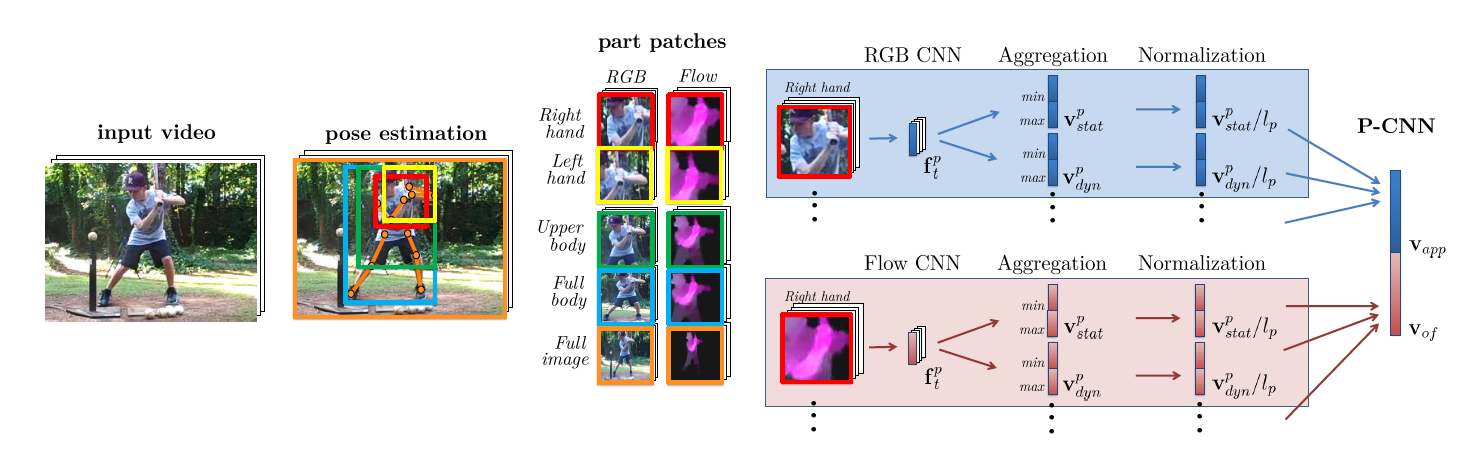
\includegraphics[width=1.0\linewidth]{P-CNN}
	\end{center}
	\caption{P-CNN features. From left to right: Input video. Human pose and corresponding human body parts for one frame
		of the video. Patches of appearance (RGB) and optical flow for human body parts. One RGB and one flow CNN descriptor $f^{p}_{t}$ is extracted per frame \textit{t} and per part \textit{p} (an example is shown for the human body part \textit{right hand}). Static frame descriptors $f^{p}_{t}$ are aggregated over time using \textit{min} and \textit{max} to obtain the video descriptor $v^{p}_{stat}$. Similarly, temporal differences of $f^{p}_{t}$ are aggregated to $v^{p}_{dyn}$. Video descriptors are normalized and concatenated over parts \textit{p} and aggregation schemes into appearance features $v_{app}$ and flow features $v_{of}$. The final P-CNN feature is the concatenation of $v_{app}$ and $v_{of}$. }
	\label{fig:pcnn}
\end{figure*}

\section{Related work}
\label{related-work}
Action Recognition in the last decade has been dominated by local and hand crafted features. In particular, Dense Trajectories (DT) features\cite{wang2013action} combined with Fisher Vector (FV)\cite{perronnin2010improving} aggregation have shown magnificent results for many challenging benchmarks.

The latest breakthroughs in Convolutional Neural Networks (CNN) have impacted a significant progress in image classification and other vision tasks.Although the applications of CNNs to action recognition in video\cite{simonyan2014two,yue2015beyond} has shown only limited improvements so far. P-CNN approach extend previous global CNN methods and address action recognition using CNN descriptors at the local level of human body parts.

Most of the recent methods for action recognition deploy global aggregation of local video descriptors. Such representations provide invariance to numerous variations
in the video but may fail to capture important spatio-temporal structure. For fine-grained action recognition, previous methods represented person-object interactions by joint tracking of hands and objects\cite{ni2014multiple} or, by linking
object proposals\cite{zhou2015interaction}. Alternative methods represent action using positions and temporal difference of body joints. Hence, it seems that Pose Estimation is a very important task for action recognition;however, reliable human pose estimation is still a challenging task. A recent study \cite{jhuang2013towards} reports significant gains provided by dynamic human pose features in case of the availability of reliable pose estimation. P-CNN extend the work \cite{jhuang2013towards} and designed a new CNN-based representation for human actions combing positions, appearance and motion of human joints.

\section{P-CNN: Pose-based CNN features}
\label{pcnn-features}

In \cite{cheron2015p}, they claim that human pose is essential for action recognition. They use positions of body joints to define informative image regions. Moreover, such regions are represented with motion-based and appearance-based CNN descriptors. Such descriptors
are extracted at each frame and then aggregated over time
to form a video descriptor, see figure \ref{fig:pcnn} for an overview.\\
The details are explained below.

To generate P-CNN features, optical flow is computed for each consecutive pair of frames using \cite{brox2004high} method. They borrow inspiration from \cite{gkioxari2015finding}, the values of the motion field $v_{x},v_{y}$ are transformed to the interval [0,255] by $\tilde{v}_{x|y} = av_{x|y} + b$ where $a=16$ and $b=128$. The values below 0 and above
255 are truncated. The transformed flow maps are saved as images with three channels corresponding to motion $\tilde{v}_{x|y}$ and the flow magnitude.
Given a video frame and the corresponding positions of
body joints, the RGB patches and flow patches are cropped for the following body parts: \textit{right hand, left hand, upper body, full body and full image} as illustrated in Figure\ref{fig:pcnn}. Each patch is resized to 224 x 224 pixels to match the CNN input layer. To represent appearance and motion patches, Two distinct CNNs are used with architecture similar to AlexNet\cite{krizhevsky2012imagenet}. Both networks contain 5 convolutional and 3 fully-connected layers. The output of the second fully-connected layer with $k = 4096$ values is used as a frame descriptor ($f^{p}_{t}$). For RGB patches,they use the publicly available “VGG-f” network from \cite{chatfield2014return} that has been pre-trained on the ImageNet ILSVRC-2012 challenge dataset. Regarding the flow patches, the motion network provided by \cite{gkioxari2015finding} are being used which was pre-trained for action recognition task on the you tube video UCF101 dataset. \\
Given descriptors $f^{p}_{t}$ for each part \textit{p} and each frame \textit{i} of video, the proceeding step is to aggregate $f^{p}_{t}$ over all frames to obtain a fixed-length video descriptor. They consider the \textit{min} and \textit{max} aggregation by computing the minimum and maximum values for each descriptor \textit{i} over \textit{T} video frames
\begin{align} \label{eq1}
	\begin{split}
		m_{i} &= \min_{1 \leq t \leq T} f^{p}_{t}(i), \\
		M_{i} & = \max_{1 \leq t \leq T} f^{p}_{t}(i)
		\end{split}
\end{align}
The static video descriptor for part p is defined by the concatenation of time-aggregated frame descriptors as
\begin{equation} \label{eq2}
	v^{p}_{stat} = [m_{1},...,m_{k},M_{1},...,M_{k}]^{T}.
\end{equation}
To capture temporal evolution of per-frame descriptors, the temporal differences will be in form $\displaystyle \Delta f^{p}_{t} = f^{p}_{t+\Delta t} - f^{p}_{t} \text{ for } \Delta t=4 \text{ frames}$. Similar to \eqref{eq1}, the aggregation of temporal differences values is computed for minimum $\Delta m_{i}$ and maximum  $\Delta m_{i}$ of $\Delta f^{p}_{t}$ and concatenate them into the dynamic video descriptor
\begin{equation} \label{eq3}
v^{p}_{stat} = [\Delta m_{1},...,\Delta m_{k},\Delta M_{1},...,\Delta M_{k}]^{T}.
\end{equation}
Finally, video descriptors for motion and appearance for all
parts and different aggregation schemes are normalized and
concatenated into the P-CNN feature vector. The normalization
is performed by dividing video descriptors by the
average $L_{2-norm}$ of the $f^{p}_{t}$ from the training set.The concatenation of static and dynamic descriptors will be denoted by “Static+Dyn”.\\
The final dimension of our P-CNN is $(5x4x4K)x 2 = 160K$, i.e., 5 body parts, 4 different aggregation schemes, 4K-dimensional CNN descriptor for appearance and motion. P-CNN training is performed using a linear SVM.
%------------------------------------------------------------------------
\section{IPCNN: Improved P-CNN}
\label{ipcnn}
In the previous section, we discussed the details of the P-CNN approach which is in brief extracting the video descriptors $V^{p}_{Static+Dyn}$ for each body part p aggregated across all the frames. The frame descriptor $f^{p}_{t}$ is computed from the appearance-based and motion-based CNNs pre-trained models. In this section, we will discuss the improved version of P-CNN which is replacing the "VGG-F" apperance CNN with the state of art image classification very Deep CNN called Deep Network(ResNet)\cite{he2015deep}.

According to ImageNet 2015, ResNet out performs all the other approaches like GoogleNet\cite{szegedy2015going} and Vgg-f as illustrated in figure \ref{fig:imagenet}.An ensemble of these residual nets achieves 3.57\% error on the ImageNet test set. This result won the 1st place on the ILSVRC 2015 classification task. On the ImageNet dataset they evaluated residual nets with a depth of up to 152 layers-8x deeper than VGG nets but still having lower complexity. Hence, it is proven that deeper net is better performance in case there is no degradation problem and ResNet is a stack of residual blocks with very deep architecture that solves the vanishing gradients problem, see figure \ref{fig:resnet}.

In the context of action recognition and P-CNN method, we apply the same approach on JHMDB dataset\ref*{dataset} by replacing "VGG-F" appearance-based model with ResNet-50 (50 layers Residual Blocks). In contrast with \ref{pcnn-features}, the output of the last average pooling layer with k=2048 values is used as appearance frame descriptor $f^{p}_{t}$. This improved version of P-CNN (IP-CNN) out performs the original approach by 3~4\%; for more details read section \ref{results}.

\begin{figure}
	\begin{center}
		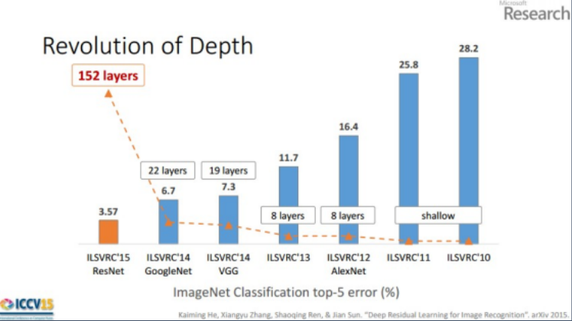
\includegraphics[width=1.0\linewidth]{resnet_imagenet}
	\end{center}
	\caption{Performance of different approaches in ImageNet 2015 competition.}
	\label{fig:imagenet}
\end{figure}

\begin{figure}
	\begin{center}
		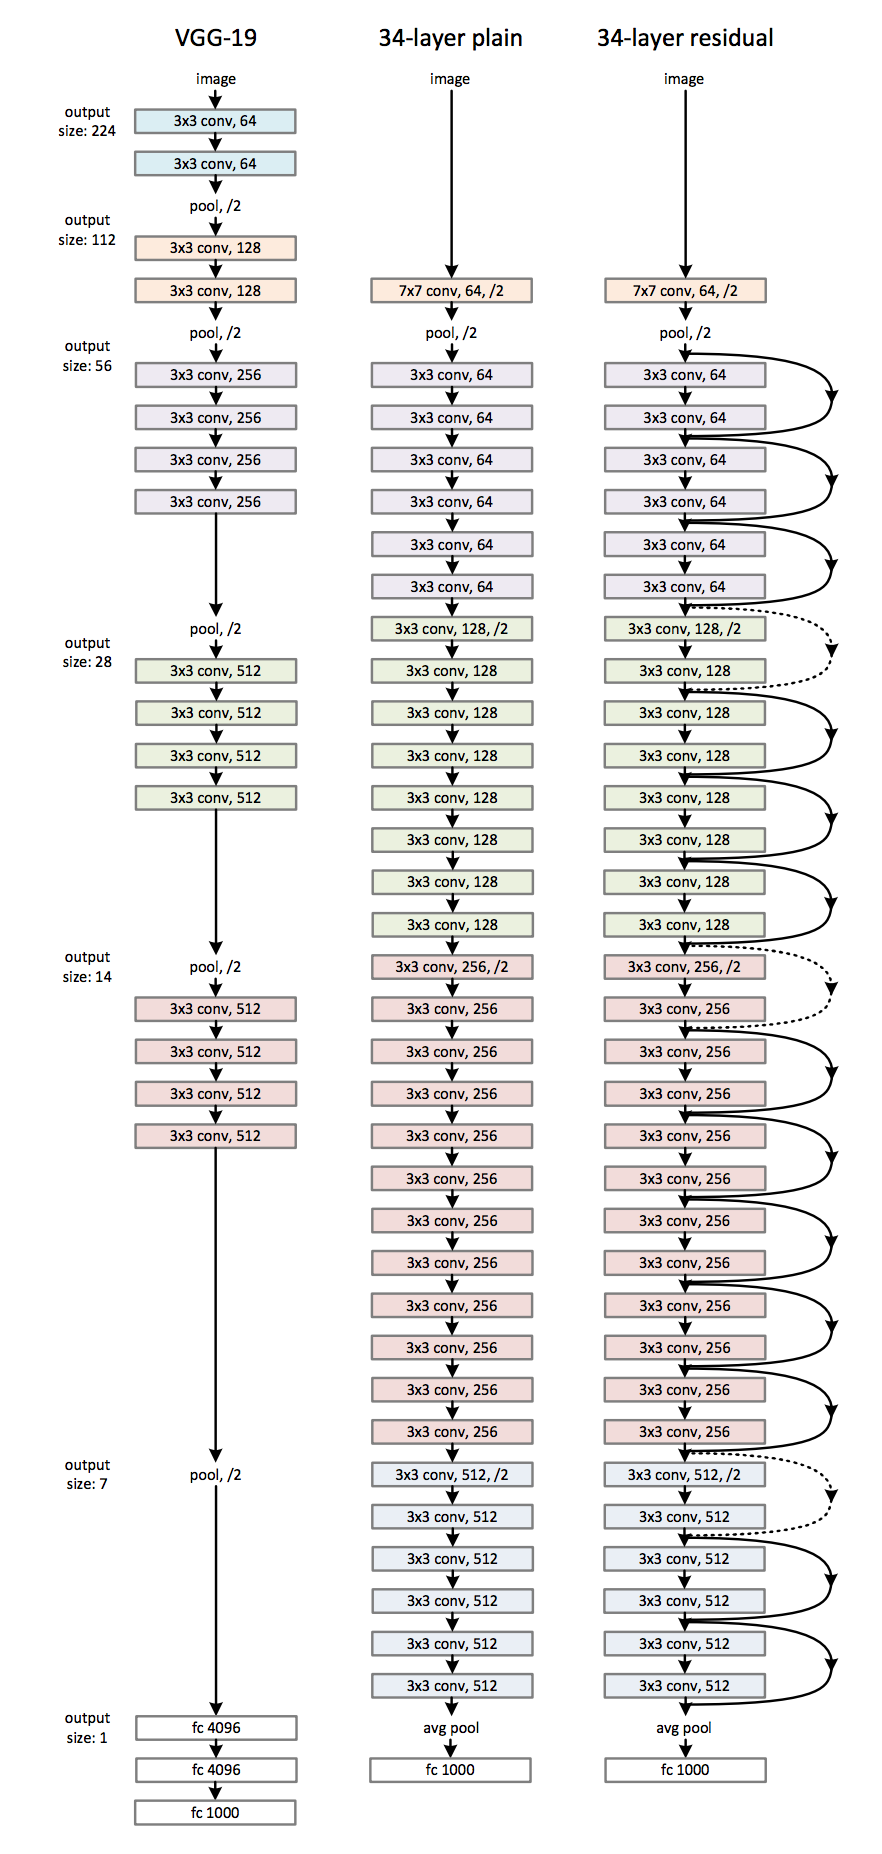
\includegraphics[width=1.0\linewidth]{resnet}
	\end{center}
	\caption{Example network architectures for ImageNet. Left: the
		VGG-19 model (19.6 billion FLOPs) as a reference. Middle:
		a plain network with 34 parameter layers (3.6 billion FLOPs).
		Right: a residual network with 34 parameter layers (3.6 billion
		FLOPs). The dotted shortcuts increase dimensions. }
	\label{fig:resnet}
\end{figure}

\section{P-CNN without Pose Estimation}

In this section, we want to prove that the claim in \cite{cheron2015p} regarding the importance of the human pose in the action recognition task is correct. Removing the pose information from the patch extraction process and use another naive approach will prove by contradiction how crucial the human joints positions to the task. 

In \cite{cheron2015p}, they compared P-CNN using ground truth pose to the automatic pose estimation; the summary of the results is shown in Table \ref{table:pose}. On the other hand, we tried different approaches for parts extraction without using the pose information.The first approach named "NoPose" is to crop an image into quarters and a center one regardless the human bounding box and the second approach "NoPose-BB" is similar to the previous one but extract the crops within the human bounding box;see figure \ref{fig:nopse}. The results have proven the claim of the importance of human pose in our task and this will be discussed in Section \ref{results}.

\begin{table}
	
	\begin{center}
		\begin{tabular}{cccc}
			\hline
			& & JHMDB\\ [0.5ex] 
			\cline{2-4}
			 & GT & Pose\cite{cherian2014mixing} & diff \\ [0.5ex]
			\hline
			P-CNN & 74.6 & 66.8 & 13.5\\
			HLPF  & 77.8 & 25.3 & 52.5\\
			\hline
		\end{tabular}
	\end{center}
	\caption{Impact of automatic pose estimation versus
		ground-truth pose (GT) for P-CNN features and HLPF\cite{jhuang2013towards}.Results are presented for JHMDB (\% accuracy )}
	\label{table:pose}
\end{table}

\begin{figure}
	\begin{center}
		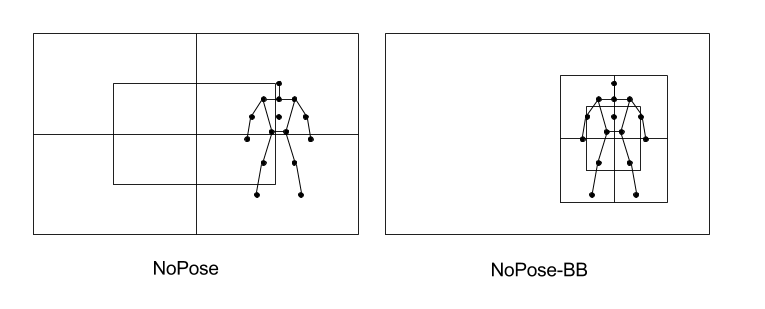
\includegraphics[width=1.0\linewidth]{nopose}
	\end{center}
	\caption{Illustration of the cropping approaches without Pose information. \textbf{\textit{NoPose}} : crops of an image subdivided in quarters and a center crop regardless the human bounding box. \textbf{\textit{NoPose-BB}}:  similar to \textit{NoPose} but within the human bounding box.}
	\label{fig:nopse}
\end{figure}
%-------------------------------------------------------------------------
\section{Datasets}
\label{dataset}
In our experiments, we use a well-known dataset called JHMDB (Joint-annotated Human Motion Data Base)\cite{jhuang2013towards}. We present it in the following.
\paragraph{JHMDB}is a subset of \textbf{HMDB}\cite{kuehne2011hmdb}, see figure \ref{fig:JHMDB}. It contains 21 human actions, such as \textit{brush hair, climb, golf, run or sit}. Video clips are restricted to the duration of the action. There are between 36 and 55 clips per action
for a total of 928 clips. Each clip contains between 15 and
40 frames of size 320 X 240. Human pose is annotated in each of the 31838 frames. There are 3 train/test splits for the JHMDB dataset and evaluation averages the results over these three splits. The metric used is accuracy: each clip
is assigned an action label corresponding to the maximum value among the scores returned by the action classifiers.

\begin{figure}
	\begin{center}
		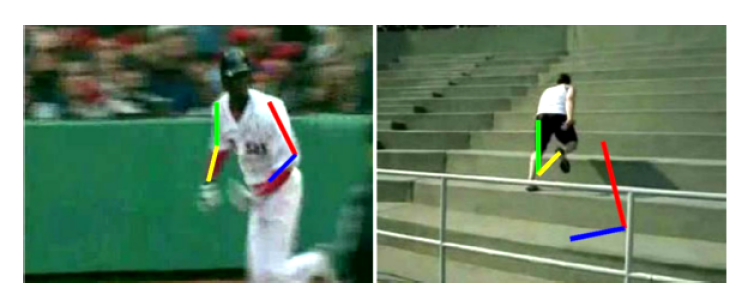
\includegraphics[width=1.0\linewidth]{JHMDB}
	\end{center}
	\caption{Examples from JHMDB dataset}
	\label{fig:JHMDB}
\end{figure}


%-------------------------------------------------------------------------
\section{Experimental results}
\label{results}
This section describes our experimental results and highlight important experiments done on the original approach in \cite{cheron2015p}. First, we present the evaluation of the complementarity of different human parts in Section\ref{diffParts}. We then compare the performance of the Original P-CNN and our improved P-CNN with ResNet in Section\ref{resnetVsvgg}. 

\subsection{Performance of human part features}
\label{diffParts}
\begin{table}
	
	\begin{center}
		\begin{tabular}{cccc}
			\hline
			& & JHMDB-GT\\ [0.5ex] 
			\cline{2-4}
			Parts & App & OF & App + OF \\ [0.5ex]
			\hline
			Hands & 46.3 & 54.9 & 57.9\\
			Upper body  & 52.8 & 60.9 & 67.1\\
			Full body  & 52.2 & 61.6 & 66.1\\
			Full body  & 43.3 & 55.7 & 61.0\\
			All  & \textbf{60.4} & \textbf{69.1} & \textbf{73.4}\\
			\hline
		\end{tabular}
	\end{center}
	\caption{Performance of appearance-based (App) and flow-based (OF) P-CNN features. Results are obtained with maxaggregation for JHMDB-GT (\% accuracy)}
	\label{table:diffparts}
\end{table}

Table \ref{table:diffparts} compares the performance of human part CNN features for both appearance and flow on JHMDB-GT (the JHMDB dataset with ground-truth pose). We can observe that all human parts (hands, upper body, full body) as well as the full image have similar performance and that their combination improves the performance significantly. We can also observe that flow descriptors consistently outperform appearance descriptors by a significant margin for all parts as well as for the overall combination \textit{All}. Moreover, we can observe that the combination of appearance and flow further improves the performance for all parts including their combination \textit{All}. This is the pose representation used in the rest of the evaluation.


\subsection{Performance of different pre-trained CNN models (Vgg-f vs ResNet)}

As explained in Section \ref{resnetVsvgg}, our proposal for improvement was replacing the vgg-f cnn with ResNet-50 for appearance-based descriptors. The experiment shows an outstanding results which is summarized in table \ref{table:resnet}. The comparsion is between the oringal P-CNN approach (App + OF) and the improved P-CNN (ResNet-50 + OF). We can observe that IP-CNN outperforms the normal method due to the usage of ResNet as the appearance CNN model descriptor. As explained before, ResNet nowadays is the state of art for the image classification task and since deeper is better then we should expect that results. 

\begin{table}
	
	\begin{center}
		\begin{tabular}{ccc}
			& App + OF & ResNet-50 + OF \\ [0.5ex]
			\hline
			& 74 & \textbf{77}\\
			\hline
		\end{tabular}
	\end{center}
	\caption{P-CNN vs IP-CNN on JHMDB(\% accuracy)}
	\label{table:resnet}
\end{table}
\label{resnetVsvgg}
{\small
\bibliographystyle{ieee}
\bibliography{egbib}
}

\end{document}
